\documentclass[12pt,twoside]{article}

%Packages
\usepackage[utf8]{inputenc}
\usepackage{amssymb}
\usepackage{amsmath}

\usepackage{enumerate}
\usepackage{tabularx,booktabs,mathrsfs,setspace}%
\usepackage{mathtools}
\usepackage{enumerate}
\usepackage{graphicx}
\usepackage{caption}
\usepackage[a4paper,top=20mm,bottom=20mm,left=20mm,right=20mm]{geometry}
\usepackage{appendix} % Add this line to define the "appendices" environment

% Algorithm
\usepackage{algorithm}
\usepackage{algorithmic}

% For longtable
\usepackage{longtable}
\usepackage{booktabs}
\renewcommand{\arraystretch}{1}
\setlength{\tabcolsep}{3pt}

% % For svg
% \usepackage{svg}

% ++++++++++++++++++++++++++Code global config begin++++++++++++++++++++++++++
% Code block universal settings, all lstdefinestyle must appeared below this block!
\usepackage{listings}
% use txtt global font
\usepackage[T1]{fontenc} % Add font options
\DeclareFixedFont{\codefont}{T1}{txtt}{m}{n}{12} % other options: txtt -> cmtt, pcr, fvm, zi4; m -> bx, n; 12 -> (fontsize)

% Define colors
\usepackage{color}
\usepackage{tikz} % colorlet need this
\definecolor{commentgreen}{rgb}{0,0.5,0}
\colorlet{framegray}{black!40}
\definecolor{stringred}{rgb}{0.6,0,0}

% Global config
\lstset{
    backgroundcolor=\color{gray!7},
    numbers = left, % show line number on the left
    numberstyle = \small\color{framegray}, % line number color
    basicstyle = \codefont, % code font
    columns = flexible, % make the spacing between characters compact
    keepspaces = true,  % keeps spaces in text, useful for keeping indentation of code (needs columns=flexible)
    % captionpos = b, % caption at the bottom
    commentstyle = \color{commentgreen}, % comment color
    frame = single, % display frame
    stringstyle = \color{stringred}, % Strings in red
    rulecolor = \color{framegray}, % frame color
    showstringspaces = false, % don't mark spaces in strings
    breaklines = true, % break long lines
    tabsize = 4, % tab size
}
% +++++++++++++++++++++++++++Code global config end+++++++++++++++++++++++++++

% ++++++++++++++++++++++++++Bash local config begin++++++++++++++++++++++++++
% Must placed below the global settings
% this will override the global settings
\lstdefinestyle{custombash}{
    language = bash,
    basicstyle = \ttfamily, % Monospaced font
    keywordstyle = \color{blue}\bfseries, % Keywords in bold blue
    stringstyle = \color{green}, % Strings in green
    commentstyle = \color{gray}, % Comments in gray
    morekeywords = {sudo, ls, cd, rm, mkdir}, % Add common Bash commands
}
% +++++++++++++++++++++++++++Bash local config end+++++++++++++++++++++++++++

% ++++++++++++++++++++++++++Python local config begin++++++++++++++++++++++++++
% Must placed below the global settings
% Custom colors for python only
\definecolor{emphblue}{rgb}{0,0,0.5}
\definecolor{keywordpink}{RGB}{128, 0, 128}
% this will override the global settings
\lstdefinestyle{custompython}{
    language = Python,
    emph = {__init__}, % Custom highlighting
    emphstyle = \color{emphblue},  % Highlighted words in deepblue
    keywordstyle = \color{keywordpink},
    upquote = true, % single quotes in straight quote
}
% ++++++++++++++++++++++++++++Python local config end++++++++++++++++++++++++++++



\begin{document}


\tableofcontents


\listoffigures
\listoftables
\newpage

\begin{abstract}
    In this article, we presented a new lossless coding scheme called 2nd-order Adaptive Markov Encoding (2nd-ord AME, abbreviated AME) coding and evaluated the overall performance when combined with huffman coding and fano coding.
\end{abstract}

\section{Introduction}
Huffman coding is one of the most well-known source coding methods, proposed by David A. Huffman in 1952. It is a coding method based on the greedy algorithm, capable of generating an optimal prefix code for a given set of symbols, ensuring that the length of each symbol’s code is inversely proportional to its probability of occurrence. The advantages of Huffman coding lie in its efficiency and optimization: it dynamically generates the optimal code based on the frequency of symbols and ensures uniquely decodable codes \cite{ref2, ref3}.

\section{Compression is Equivalent to Prediction}

In this section, we state the motivation behind AME coding. 

Both huffman coding and fano coding are based on the assumption that the source is \textit{discrete memoryless}. They are trying to approach the compression limit (which is the entropy of the source \cite{ref1}) given that the original source looks random. So they are called ``entropy coding''. However, in practice, the texts inherently take some structures that cannot be explicitly captured by any relative simple models. These structures are not considered when performing entropy coding, so we wasted some potential compression ratio.

No matter what coding method we choose, like LZ77, (need more), the last step them is always entropy coding. But entropy coding is well-understood and mature (Huffman being the ``optimal'' in some sense). Therefore, the only way to improve compression ratio is to uncover the structure of the source. We need to design a better model first to capture and hiding those structures while exposing the true ``memoryless components'' of the source, then the utility of entropy coding can be maximized.

The basic idea behind AME coding is that compression is equivalent to \textit{prediction}. We are essentially building a same text predictor in both sides of the transmitter and the receiver. As long as the predicted next character matches the true one, that character is not considered as the ``memoryless component'' of the source (it depends on the history text). But if the predicted one doesn't match the true one, this means there are somewhat ``random'' factors come into play. If we can proposed some encoding strategy that makes the predictor works exactly the same on both the transmitter and receiver, we only need to transmit the ``memoryless components'' and the number of correct predictions. 

For example, if we want to extract the ``memoryless components'' of the following content:

% literal bash commands
\begin{lstlisting}[language=bash, style=custombash]
Information theory is interesting.
\end{lstlisting}

Feed it into the predictor, suppose we can correctly predict the character in position 2, 5-11, 15-19, 21-22, 26-34, we only need to transmit the initial letter that cannot be predicted together with the number of correct predictions:

\begin{lstlisting}[language=bash, style=custombash]
I1fo7 th5i2int9
\end{lstlisting}

The rest letters are somehow losed some internal dependence and can be approximately considered as memoryless. 

We can see in this example the efficiency of compression directly relies on how well we extract the ``memoryless components'' of the text, in other words, the performance of the predictor. Since human language is the product of human mind, which definitely cannot be modelled using just a few parameters. An accurate predictor would need millions of parameters, which is essentially a neural network. However, due to time and space complexity, using a neural network to predict the next character is not feasible in practice. However, we can use a simpler model called markov chain to capture some of the structures in the text.

\section{Mechanism of AME Coding}

We assume no prior knowledge of the source. So the predictor is built simultaneously with the encode/decode process. The algorithm for AME encoding and decoding are shown in Algorithm~\ref{alg:markov_encode} and \ref{alg:markov_decode}. The codes are written in Python and can be found in the appendix~\ref{app:markov_encode} and \ref{app:markov_decode}.

\begin{algorithm}
    \caption{Adaptive Markov Encoding}
    \label{alg:markov_encode}
    \begin{algorithmic}[1]
    \REQUIRE Input file \texttt{source.txt}, Output file \texttt{markov\_encoded.txt}
    \ENSURE Encoded text stored in \texttt{markov\_encoded.txt}
    \STATE Initialize an empty tree \texttt{tree}, list \texttt{encoded\_output}, and counter \texttt{correct\_predictions = 0}
    \STATE Read \texttt{source\_text} from \texttt{source.txt}
    \FOR{\texttt{i = 1} to \texttt{length(source\_text)}}
        \STATE \texttt{current\_char = source\_text[i]}
        \IF{\texttt{i == 1}} 
            \STATE Append \texttt{current\_char} to \texttt{encoded\_output}
            \STATE Add root-to-\texttt{current\_char} transition to \texttt{tree}
        \ELSE
            \STATE Predict next character using \texttt{tree}: \texttt{prediction = predict\_next(tree, prev\_char)}
            \IF{\texttt{prediction == current\_char}}
                \STATE Increment \texttt{correct\_predictions}
            \ELSE
                \IF{\texttt{correct\_predictions > 0}}
                    \STATE Append \texttt{correct\_predictions} to \texttt{encoded\_output}
                    \STATE Reset \texttt{correct\_predictions = 0}
                \ENDIF
                \STATE Append \texttt{current\_char} to \texttt{encoded\_output}
            \ENDIF
            \STATE Add transition \texttt{prev\_char $\to$ current\_char} to \texttt{tree}
        \ENDIF
        \STATE \texttt{prev\_char = current\_char}
    \ENDFOR
    \IF{\texttt{correct\_predictions > 0}}
        \STATE Append \texttt{correct\_predictions} to \texttt{encoded\_output}
    \ENDIF
    \STATE Write \texttt{encoded\_output} to \texttt{markov\_encoded.txt}
    \end{algorithmic}
\end{algorithm}

\begin{algorithm}
    \caption{Adaptive Markov Decoding}
    \label{alg:markov_decode}
    \begin{algorithmic}[1]
    \REQUIRE Input file \texttt{markov\_encoded.txt}, Output file \texttt{markov\_decoded.txt}
    \ENSURE Decoded text stored in \texttt{markov\_decoded.txt}
    \STATE Initialize an empty tree \texttt{tree}, list \texttt{decoded\_output}
    \STATE Read \texttt{encoded\_text} from \texttt{markov\_encoded.txt}
    \STATE \texttt{i = 1}
    \WHILE{\texttt{i $\leq$ length(encoded\_text)}}
        \STATE \texttt{current\_char = encoded\_text[i]}
        \IF{\texttt{i == 1}}
            \STATE Append \texttt{current\_char} to \texttt{decoded\_output}
            \STATE Add root-to-\texttt{current\_char} transition to \texttt{tree}
        \ELSE
            \STATE \texttt{prev\_char = decoded\_output[last]}
            \IF{\texttt{current\_char} is a digit}
                \STATE Extract full number as \texttt{repeat\_count}
                \STATE Predict next character using \texttt{tree}: \texttt{prediction = predict\_next(tree, prev\_char)}
                \FOR{\texttt{j = 1} to \texttt{repeat\_count}}
                    \STATE Append \texttt{prediction} to \texttt{decoded\_output}
                    \STATE Add transition \texttt{prev\_char $\to$ prediction} to \texttt{tree}
                    \STATE \texttt{prev\_char = prediction}
                \ENDFOR
            \ELSE
                \STATE Append \texttt{current\_char} to \texttt{decoded\_output}
                \STATE Add transition \texttt{prev\_char $\to$ current\_char} to \texttt{tree}
            \ENDIF
        \ENDIF
        \STATE \texttt{i = i + 1}
    \ENDWHILE
    \STATE Write \texttt{decoded\_output} to \texttt{markov\_decoded.txt}
    \end{algorithmic}
\end{algorithm}


\section{Entropy Coding Review}

\subsection{Mechanism of Huffman coding}
\label{sec:huffman}


\subsection{Mechanism of Fano coding}

\section{Implementation}

We performed two seperated experiments for different purposes. The first is to realize Huffman and Fano coding on the original text and perform evaluations. The second is to combine AME coding with Huffman and Fano coding and evaluate the performance of the new scheme.

\subsection{Without AME}

The encode/decode process in shown in the form of a flowchart shown in Figure~\ref{fig:without-ame}.

\begin{figure}[h!]
    \centering
    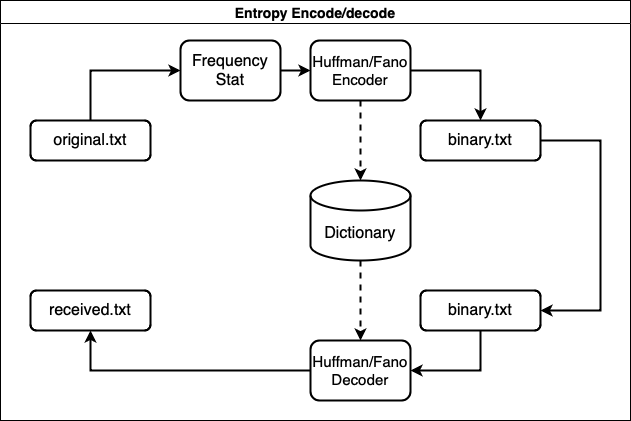
\includegraphics[width=0.7\textwidth]{without-ame.png}
    \caption{Flowchart of the experiment without AME}
    \label{fig:without-ame}
\end{figure}

The content in \texttt{original.txt} contains the first three chapters of \textit{the Game of Thrones}. Part of the \texttt{original.txt} is shown in Appendix~\ref{lst:originalpart}.

In order to perform huffman/fano coding on the text, we first need to calculate the frequency of each character in the text. The frequency of each character is shown in Table~\ref{tab:frequency}.

\begin{longtable}{ccc||ccc||ccc}
    \caption{Frequency of each character in \texttt{original.txt}}
    \label{tab:frequency} \\
    \toprule
    \textbf{Index} & \textbf{Symbol} & \textbf{Probability} & \textbf{Index} & \textbf{Symbol} & \textbf{Probability} & \textbf{Index} & \textbf{Symbol} & \textbf{Probability} \\ \hline
    \endfirsthead
    \hline
    \textbf{Index} & \textbf{Symbol} & \textbf{Probability} & \textbf{Index} & \textbf{Symbol} & \textbf{Probability} & \textbf{Index} & \textbf{Symbol} & \textbf{Probability} \\ \hline
    \endhead
    \hline
    \endfoot
    1 & (LF) & 0.0052 & 2 & (CR) & 0.0052 & 3 & (Space) & 0.1915 \\ 
    4 & ! & 0.00020423 & 5 & , & 0.0127 & 6 & - & 0.001 \\ 
    7 & . & 0.0165 & 8 & 1 & 2.0423e-05 & 9 & 2 & 2.0423e-05 \\ 
    10 & : & 4.0846e-05 & 11 & ; & 0.00024507 & 12 & ? & 0.002 \\ 
    13 & A & 0.0013 & 14 & B & 0.0017 & 15 & C & 0.00055141 \\ 
    16 & D & 0.00036761 & 17 & E & 0.00038803 & 18 & F & 0.00079649 \\ 
    19 & G & 0.0011 & 20 & H & 0.0024 & 21 & I & 0.0026 \\ 
    22 & J & 0.001 & 23 & K & 0.00020423 & 24 & L & 0.00055141 \\ 
    25 & M & 0.00051057 & 26 & N & 0.0011 & 27 & O & 0.00046972 \\ 
    28 & P & 0.00022465 & 29 & R & 0.0017 & 30 & S & 0.0014 \\ 
    31 & T & 0.0037 & 32 & U & 0.00014296 & 33 & V & 8.1691e-05 \\ 
    34 & W & 0.0034 & 35 & Y & 0.00061268 & 36 & a & 0.0585 \\ 
    37 & b & 0.0109 & 38 & c & 0.0135 & 39 & d & 0.0414 \\ 
    40 & e & 0.0959 & 41 & f & 0.0156 & 42 & g & 0.016 \\ 
    43 & h & 0.052 & 44 & i & 0.0435 & 45 & j & 0.00061268 \\ 
    46 & k & 0.0079 & 47 & l & 0.035 & 48 & m & 0.0154 \\ 
    49 & n & 0.0476 & 50 & o & 0.0546 & 51 & p & 0.0079 \\ 
    52 & q & 0.0004493 & 53 & r & 0.0451 & 54 & s & 0.0475 \\ 
    55 & t & 0.0606 & 56 & u & 0.0174 & 57 & v & 0.0051 \\ 
    58 & w & 0.0192 & 59 & x & 0.00028592 & 60 & y & 0.0139 \\ 
    61 & z & 0.00036761 & 62 & ’ & 0.0026 & 63 & “ & 0.0051 \\ 
    64 & ” & 0.0051 & 65 & . & 4.0846e-05 &  &  &  \\ 
    \toprule
\end{longtable}

According to the frequency of each character, we can create the Huffman tree based on the methods in Section~\ref{sec:huffman} and generate the huffman dictionary, which is shown in 



First, we applied the Huffman coding to the first three chapters of \textit{the Game of Thrones} and calculate related 4 main parameters, including the average code length $\bar{L}$, code rate $k$, efficiency $\eta$, and compression ratio $\xi$.





Given that Huffman coding is the optimal method for generating codes, especially when there are significant differences in the probabilities of occurrence for different source symbols, it significantly outperforms the Fano coding technique in terms of coding effectiveness \cite{ref3, ref4}. Therefore, we designed an exploratory section in which we applied the Fano coding technique to perform the same operations on the target text and compared the calculated parameters with those obtained using the Huffman coding technique.

\subsection{With AME}

The experiment procedure of the encode/decode process in shown in Figure~\ref{fig:with-ame}.

\begin{figure}[h!]
    \centering
    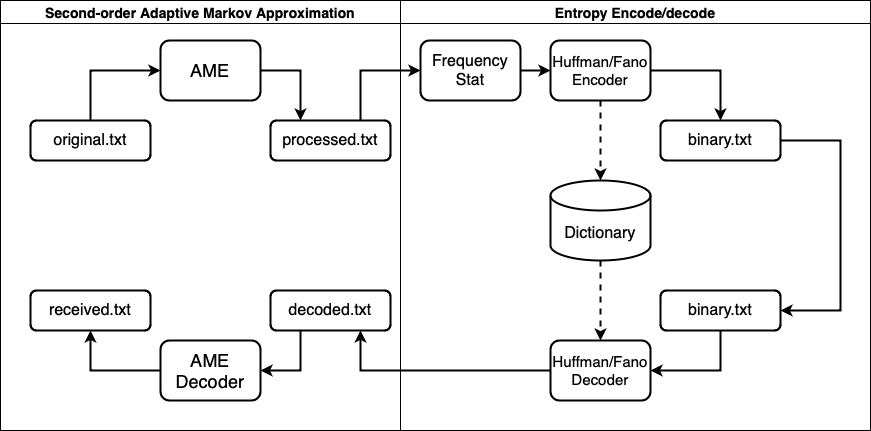
\includegraphics[width=0.8\textwidth]{with-ame2.png}
    \caption{Flowchart of the experiment with AME}
    \label{fig:with-ame}
\end{figure}



\section{Results and Discussion}

\section{Conclusion}


\begin{thebibliography}{9}
    \bibitem{ref1} C. E. Shannon, “A Mathematical Theory of Communication”.

    \bibitem{ref2} Advances in Communication and Computing Technologies (ICACACT 2014), Mumbai, India, 2014, pp. 1-6, doi: 10.1109/EIC.2015.7230711.

    \bibitem{ref3} N. Dhawale, ``Implementation of Huffman algorithm and study for optimization,'' 2014 International Conference on Advances in Communication and Computing Technologies (ICACACT 2014), Mumbai, India, 2014, pp. 1-6, doi: 10.1109/EIC.2015.7230711.

    \bibitem{ref4} S. Congero and K. Zeger, "Competitive Advantage of Huffman and Shannon-Fano Codes," in IEEE Transactions on Information Theory, vol. 70, no. 11, pp. 7581-7598, Nov. 2024, doi: 10.1109/TIT.2024.3417010. 

\end{thebibliography}

\newpage
\appendix

\begin{appendices}

\section{Python code for AME encoding}
\label{app:markov_encode}

\lstinputlisting[caption={AME encoder}, label={lst:markov_encode}, language=Python, style=custompython]{../markovpy/adaptive_markov_encode.py} % python

\section{Python code for AME decoding}
\label{app:markov_decode}

\lstinputlisting[caption={AME decoder}, label={lst:markov_decode}, language=Python, style=custompython]{../markovpy/adaptive_markov_decode.py} % python

\section{Part of the \texttt{original.txt}}
\label{lst:originalpart}

\lstinputlisting[language=bash, style=custombash]{original_partof.txt} % bash



\end{appendices}



\end{document}